
\section {Experimental Setup}
The setup is illustrated in Figure \ref{fig:ExperimentalSetup}.
\begin{figure}[htbp]
    \centering
    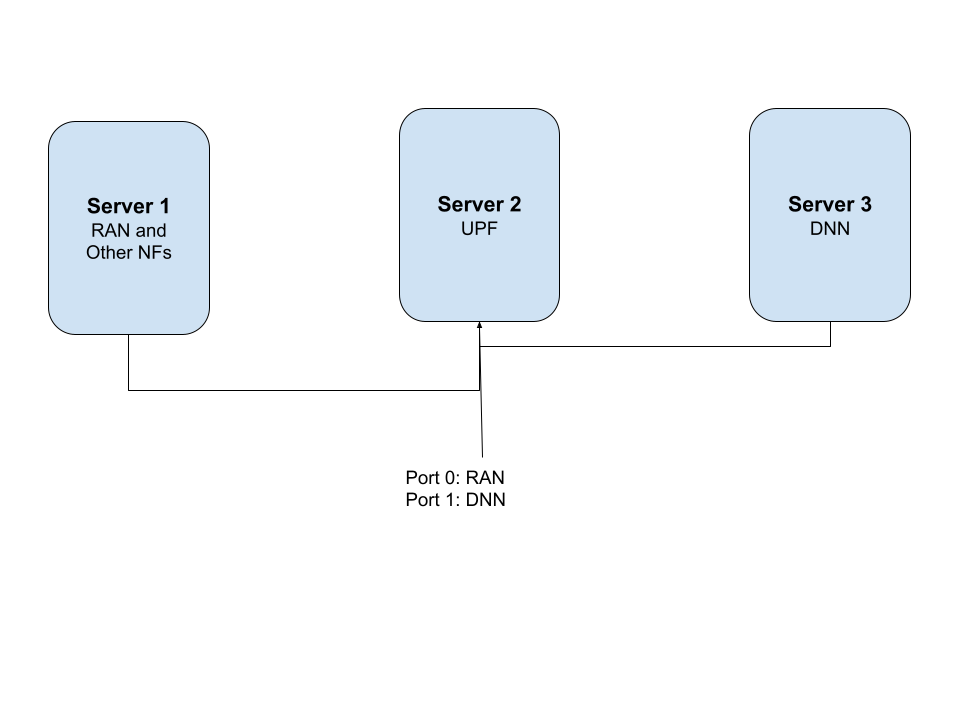
\includegraphics[width=0.7\textwidth, keepaspectratio]{./fig/Results/Setup.png}
    \caption{Experimental Setup}
    \label{fig:ExperimentalSetup}
\end{figure}
 The main features of the setup are: 
 \begin{itemize} 
        \item \textbf{Server's Layout}
        \begin{enumerate}
                \item \textbf{Server 1} The radio access network (RAN) and other network functions responsible for authentication,
         session establishment, charging functions are simulated on server 1.  The user equipments are also 
         simulated on the same machine. The load generation in the uplink direction is the main function of this server in the data forwarding plane.
                \item \textbf{Server 2} This server hosts the user plane function
		 (UPF). Two ports on this server are used to communicate with RAN 
         (server 1) and DNN (server 3).
                 \item \textbf{Server 3} This server simulates the data network name (DNN) network function. This network 
        function is the gateway to public Internet for 5G telecommunication. This server is used to generate downlink traffic. This server is also used to mirror packets received from uplink and forwarded back in the downlinj direction. The mirroring of latency packets help in measuring end-to-end latency (Round Trip Time) at the RAN. 
        \end{enumerate} 
        \item \textbf{Hardware Configuration} 
        \begin{enumerate}
                \item \textbf{CPU} Intel Xeon Core i5 @2.20GHz. 12 cores on every NUMA node. Only a single NUMA node is used in the experiments. Hyperthreading is kept off to facilitate repeatability of results.
                \item \textbf{Memory} 8192 superpages of size 2MB are reserved initially for the whole run.
                \item \textbf{Cache} 32 KB L1i-cache, 32 KB L1d-cache, 256 KB L2 cache per core. 30 MB L3 cache per NUMA node. 
                \item \textbf{NIC} Netronome Agilio CX 2x10GbE smartNIC.
	       \end{enumerate}
        
\end{itemize}

\section{UPF}
The primary role of user plane function is described in \ref{sec:5GDataPlane}. UPF is the main network function which takes the centre stage in the core network. The RAN load generator is used to test the processing capability of UPF. The metrics used are throughput and latency of data plane and control plane traffic. 

Different designs of the UPF are studied:

\begin{itemize}
	\item \textbf{Software UPF}

	This design uses kernel bypass framework DPDK for userspace processing of the incoming packets. All the control plane and data plane packets are received on the master core which redirects these packets into different worker cores.
	\item \textbf{Offloaded Data Plane}
	The complete data plane processing is offloaded on the smartNIC. The control plane messages are still processed in the software. Once a session is established (released), the rules are inserted (removed) in the smartNIC.
	
	\item \textbf{Offloaded Control Plane}
	In this design, the control plane handling is offloaded to the NIC. 
\end{itemize}
The detailed description of these designs are available in \cite{}.
\begin{table}[htbp]
\begin{scriptsize}
\begin{center}
\def\arraystretch{1.5}%  1 is the default, change whatever you need
\begin{tabular}{|p{3cm}|p{2cm}|p{2cm}|p{2cm}|}\hline 
% {\bf{Performance metric}} & {\bf{DPDK-based software UPF}} & {\bf{Dataplane offload}} & {\bf{Control plane offload}} \\ \hline 
{\bf{Performance metric}} & {\bf{SoftUPF}} & {\bf{DPOffload}} & {\bf{CPOffload}} \\ \hline 
{\bf{Throughput (messages/sec)}} & 5.1K  & 666  & 2.08M  \\ \hline
{\bf{Latency ($\mu s$)}} & 113  & 1646  & 24 \\ \hline
% {\bf{Performance per USD}} & 88  & 1 & 4.6K  \\ \hline
% {\bf{Performance per Watt}} & 40  & 1 & 41K \\ \hline
\end{tabular}
% \setlength{\abovecaptionskip}{-8pt}
% \setlength{\belowcaptionskip}{8pt}
\caption{Control plane performance.} 
% \vspace{-2mm}
\label{tab:perf-cp-offload}
\end{center}
\end{scriptsize}
\end{table}

\section{Results}
\subsection{Control Plane Performance}
The latency v/s. throughput graphs for different UPF designs  are illustrated in \ref{fig:SoftwareUPF},
\ref{fig:DPOFfload}, \ref{fig:CPOffload}. The summary of the results is shown in \ref{tab:perf-cp-offload}. The table \ref{tab:perf-cp-offload}
shows the latency around the control plane saturation. The control plane throughput is defined in terms
of sessions handled per second - the whole establishment, modification and response cycle for a given session 
is counted once.
\begin{figure}[htbp]
    \centering
    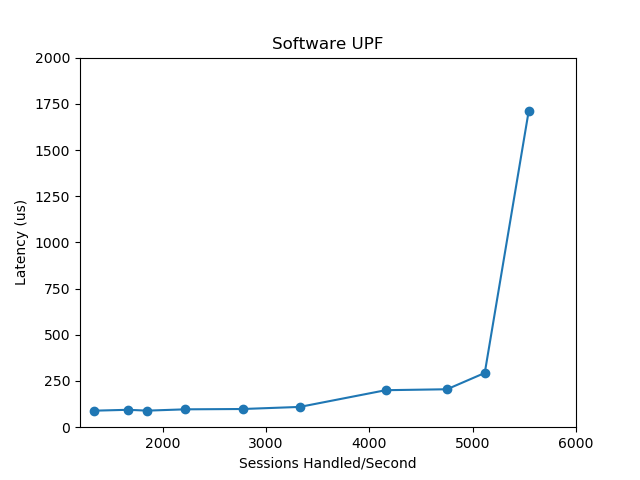
\includegraphics[width=0.7\textwidth, keepaspectratio]{./fig/Results/SoftUPF.png}
    \caption{Control Plane Performance for Software UPF}
    \label{fig:SoftwareUPF}
\end{figure}
\begin{figure}[htbp]
    \centering
    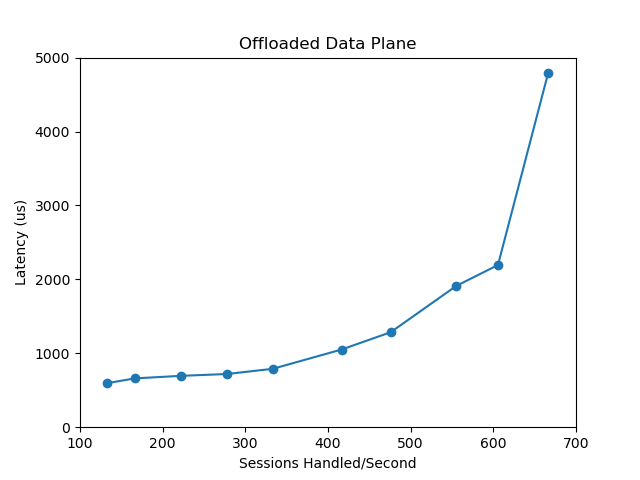
\includegraphics[width=0.7\textwidth, keepaspectratio]{./fig/Results/DPOffload.png}
    \caption{Control Plane Performance for Offloaded Data Plane}
    \label{fig:DPOFfload}
\end{figure}
\begin{figure}[htbp]
    \centering
    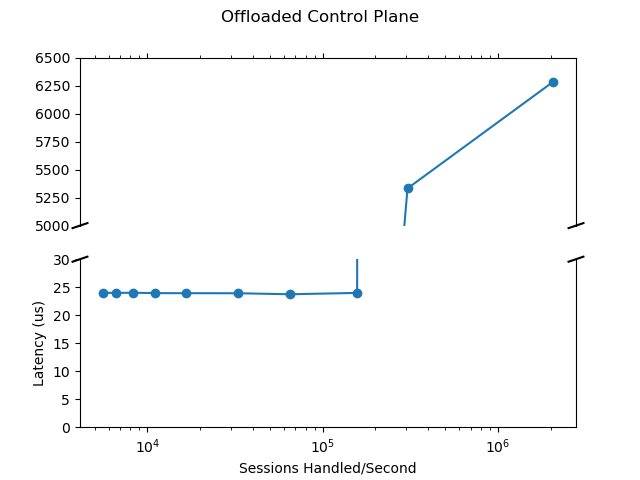
\includegraphics[width=0.7\textwidth, keepaspectratio]{./fig/Results/CPOffload.png}
    \caption{Control Plane Performance for Offloaded Control Plane}
    \label{fig:CPOffload}
\end{figure}

When the control plane is offloaded, we can see the best performance in terms of latency and throughput.
With the control plane offload, the latency is only around  24 us and 2.08 M sessions can 
be handled per second.
The performance deteriorates for data plane offload when compared to software UPF. This is 
attributed to the  bottleneck created between offloaded data plane
 and user space control plane - once the control plane messages are processed in
the user space, the rules are installed in smartNIC.
